%=========================================================================
%Jakub Bartecek (xbarte09)
%Date: 2013 - 2014
%Encoding: UTF-8
%set syntax=tex
%\listoffigures

\chapter{Úvod}
    Tento semestrální projekt se zabývá vylepšením serveru Jenkins CI, který je v praxi velmi využíván pro potřeby průběžného testování softwaru
    a jeho kontinuální integraci. Vylepšení se týká především webového serveru a \emph{servlet} kontejneru, který je v Jenkins CI integrován. 
    V současném stavu tyto funkce vykonává kombinace nástrojů Winstone a Jetty. 
    
    Server Winstone je již neudržovaný a zastaralý nástroj a z tohoto důvodu
    byl z velké části nahrazen serverem Jetty, který potřebnou funkcionalitu poskytuje. Server Jetty je poměrně komplexní projekt a nabízí
    mnoho funkcionality, ale na druhou stranu jeho rozsah nedovoluje poskytovat maximální rychlost.
    
    V současné době vznikl nový webový server Undertow, který si klade za cíl být co nejjednodušší a nejrychlejší a mohl by být přínosný
    a vhodný pro Jenkins CI. Jelikož tento server je nový a je sponzorován firmou Red Hat, tak lze předpokládat, že jeho vývoj
    bude nadále pokračovat a nebude zastarávat.

    Cílem této práce je nahradit server Jetty a případně i serveu Winstone pomocí serveru Undertow 
    a integrovat jej se serverem Jenkins CI. Při integraci je kladen důraz na snahu
    zachovat zpětnou kompatibilitu se starým řešením. 

    V rámci tohoto semestrálního projektu jsou nejprve rozebrány potřebné informace týkající se jednotlivých nástrojů a plánované integrace.
    Následně je detailně analyzována architektura Jenkins CI a způsob jeho integrace se servery Winstone a Jetty. V následující části
    je diskutována varianta nahrazení pouze serveru Jetty a varianta nahrazení serveru Jetty i Winstone pomocí serveru Undertow. 
    Z provedené analýzy je zvolena jedna varianta, která je vybrána pro následnou integraci.

    Samotná implementace integrace není předmětem tohoto semestrálního projektu a bude provedena až v navazujícím diplomovém projektu. 
    V rámci dimplomového projektu bude také provedeno testování výkonu modifikovaného systému Jenkins CI a celkové shodnocení navržených
    a provedených změn.
%TODO - že to dělám pod Red Hatem


%%%%%%%%%%%%%%%%%%%%%%%%%%%%%%%%%%%%%%%%%%%%%%%%%%%%%%%%%%%%%%%%%%%%%%%%%%%%%%%%%%%%%%%%%%%%%%%
%%%%%%%%%%%%%%%%%%%%%%%%%%%%%%%%%%%%%%%%%%%%%%%%%%%%%%%%%%%%%%%%%%%%%%%%%%%%%%%%%%%%%%%%%%%%%%%
\chapter{Jenkins CI a související nástroje}
    Tato kapitola se zaměřuje na teoretické základy práce, které je nutné nebo vhodné znát pro pochopení zpracovávané problematiky.
    Je zde detailněji popsán systém Jenkins CI (kapitola \ref{jenkins}) ke kterému se tato práce přímo váže. S ním je spojeno seznámení
    s webovými servery Winstone (kapitola \ref{winstone}) a Jetty (kapitola \ref{jetty}), jejichž kombinace je současně v Jenkins CI integrována.
    Pro tuto práci je důležité poruzumět rozdílu mezí \emph{servlet kontejnerem} a webovým server. Vysvětlením těchto pojmů se zabývá kapitola \ref{servletWebserver}.

    Větší důraz je dále věnován serveru Undertow (kapitola \ref{undertow}), který byl vybrán jako nový webový server pro Jenkins CI. V tomto případě je provedena hlubší studie
    tohoto nástroje, aby na jejím základě bylo možné pochopit a provést samotnou integraci s Jenkins CI, která je jádrem této práce. 
    Pro poskytnutí ucelených informací
    je menší prostor také vymezen pro nástroj Maven (kapitola \ref{maven}), který se používá k řízení překladu serveru Jenkins CI, a je v této práci několikrát zmiňován. 

    Uvedené informace mají spíše informativní charakter, aby poskytly ucelený úvod do zkoumané problematiky. Jsou zaměřeny především na informace týkající se samotné
    integrace. Pro případné získání detailnějších informací jsou uvedeny patřičné zdroje, kde je lze hledat.

    %%%%%%%%%%%%%%%%%%%%%%%%%%%%%%%%%%%%%%%%%%%%%%%%%%%%%%%%%%%%%%%%%%%%%%%%%%%%%%%%%%%%%%%%%%%%%%%
    \section {Jenkins CI} \label{jenkins}
        Jenkins CI je komunitní open source nástroj pro kontinuální integraci softwaru, který je vyvíjen pod svobodnou licencí
        MIT\footnote{Licence MIT: \texttt{http://opensource.org/licenses/MIT}} \cite{jenkinsGovernance}.
        Je velmi populární a využíván malými i velkými firmami jako je například firma Red Hat, kde tento program běží na stovkách serverů.
        Původní název tohoto projektu je Hudson\footnote{Webové stránky projektu Hudson: \texttt{http://hudson-ci.org/}}. 
        Když se vývoje tohoto projektu ujala firma Oracle, tak se tento projekt
        rozštěpil a vznikla komunitní verze projektu, což je server Jenkins CI. Přesto se v některých částech tohoto projektu 
        stále objevuje název Hudson, ale jedná se pouze pozůstatek z původního projektu.

        Zkratka CI je z anglického spojení \emph{continuous integration}, což lze do češtiny přeložit jako kontinuální nebo průběžná 
        integrace. Krátké seznámení se z touto metodologií je v následující kapitole.

        Informace v této kapitole byly především čerpány z knihy \cite{jenkinsBook}, kde lze nalézt další informace o serveru Jenkins CI,
        a také z webové stránky projektu \cite{jenkinsWeb}.
        %TODO přidání odkazu na vývoj servlet kontejneru v Jenkins

        \subsection{Kontinuální integrace a využití Jenkins CI}
            V minulosti byla integrace programu do výsledného produktu velmi náročným procesem a často ztraceným časem.
            S vydáním každé verze programu se musel postup probíhající před vydáním produktu opakovat a pro vývojářský tým
            to prakticky znamenalo zdržení se. Pokud se v tomto procesu odhalil nějaký problém, což bylo běžné, 
            tak jeho řešení bylo z důvodu nedostatku času a jeho pozdního objevení mnohem problematičtější,
            než kdyby byl tento problém odhalen dříve.

            Kontinuální integrace je moderní přístup k vývoji softwaru, který mění způsob myšlení nad celým procesem vývoje
            a snaží se předcházet problémům popsaným výše a především ušetřit čas. V tomto přístupu je využíván nějaký
            kvalitní nástroj, který automatizovaně provádí specifikované kroky, které provázejí integraci softwaru a jeho vydání.

            Jedním z nástrojů poskytujích podporu pro kontinuální integraci při vývoji softwaru je 
            server Jenkins CI. 
            
            \medskip \noindent Základními možnostmi, které umožňuje Jenkins CI nakonfigurovat, jsou:
            
            \begin{itemize}
                \item Spouštění integračních a jednotkových testů v přesně definovaném čase (např. v noci, kdy jsou servery méně vytížené)
                \item Spuštění integračních a jednotkových testů při změně ve verzovacím systému. Jenkins CI dokáže zaznamenat změnu v repozitáři,
                    stáhnout si změny a spustit testování
                \item Shromažďování a vyhodnocování metrik vývoje softwaru
                \item Spuštění akceptačních testů
                \item Informování e-mailem o testech, které skončily chybou
                \item Automatické nahrání nové verze produktu na server
            \end{itemize} 

            Uživatelé mohou kdykoliv přidat využití libovolné funkcionality systému a tudíž neopakovat stále stejné kroky. 
            

        \subsection{Způsoby použití aplikace}
            Celý program je napsán v jazyce Java a je tedy plně přenositelný mezi platformami. Architektura je navržena tak, aby byla 
            lehce rozšiřitelná pomocí tzv. \emph{pluginů}, kterých je pro Jenkins vytvořené velké množství. 
            
            Jenkins CI je určen pro běh na serveru a je dostupný přes webové rozhraní (ale může být samozřejmě spuštěn
            na libovolném osobním počátači). Komunikuje pomocí protokolu \emph{HTTP}, 
            který je založen na modelu \emph{požadavek-odpověď} (anglicky \emph{request-response}). Jelikož tento způsob komunikace
            je velmi běžný, tak není v programu přímo implementován, ale využívá k němu externí nástroje. 
            Dalším nástrojem, který pro svou činnost Jenkins potřebuje, je servlet kontejner ve kterém samotná 
            aplikace poběží.
            Tento pojem je blíže objasněn v kapitole \ref{servletWebserver}.

            \medskip \noindent
            Existují dvě možnosti jak spustit server Jenkins CI:

            \begin{enumerate}
                \item{Může běžet na libovolném \emph{Java EE} aplikačním serveru \cite{jenkinsServers} jako jsou například servery 
                JBoss\footnote{Více informací o serveru viz \texttt{http://www.jboss.org/jbossas/}} 
                anebo Glasfish\footnote{Více informací o serveru viz \texttt{http://www.oracle.com/technetwork/middleware/glassfish/}}}.
                Jenkins CI se standardně nasadí na server (dle zvyklostí konkrétního serveru)
                a poté je s ním možné pracovat. V tomto případě veškerou nízkoúrovňovou komunikaci pomocí \emph{HTTP} 
                i práci servlet kontejneru zajišťuje aplikační server.
                
                \item{Pokud nechceme nebo nemůžeme spouštět Jenkins CI na aplikačním serveru, tak jej lze spustit přímo
                    z vytvořené \texttt{.war} archivu (překladem se zabývá kapitola \ref{jenkinsUsage}). V tomto případě
                    se o práci servlet kontejneru i webového serveru komunikujícího protokolem \emph{HTTP} stará 
                    kombinace nástrojů Winstone a Jetty, které jsou přímo integrovány do serveru Jenkins CI. 
                    
                    Nahrazení těchto dvou nástrojů (nebo pouze serveru Jetty) a zajištění vykonávání této činnosti je hlavním cílem této práce.
                    Záměrem je tedy nahradit server Jetty a případně i server Winstone pomocí zvoleného nového serveru Undertow.
                    Studie těchto nástrojů a jejich rozbor je předmětem následujícíh kapitol.}
            \end{enumerate}

            Pro tuto práci je důležitý druhý způsob používání Jenkins CI a proto další informace se budou přímo vázat k němu.

        \subsection{Základy práce s Jenkins CI} \label{jenkinsUsage}
            Pro přeložení a spuštění aplikace je potřeba pracovat z příkazové řádky nebo provést instalaci nějakým dávkovým souborem (skriptem).
            Aplikaci je možné stáhnout připravenou přímo ze stránek projektu \cite{jenkinsWeb}, ale pro tuto práci je potřeba 
            pracovat s aplikací ze zdrojových souborů. Aktuální verze aplikace je dostupná na serveru 
            GitHub\footnote{Adresa aktuální verze Jekins CI: \texttt{www.github.com/jenkinsci}}.

            Po stažení zdrojových souborů je potřeba provést překlad aplikace. Pro tento automatizovaný překlad se používá nástroj Maven, který
            je krátce zmíněn v kapitole \ref{maven}. Pro provedení překladu bez spouštění jednotkových testů je potřeba použít tento příkaz:
            \begin{verbatim}
                mvn clean install -pl war -am -DskipTests
            \end{verbatim}
            Pokud bychom chtěli spustit jednotkové testy aplikace, tak jednoduše vynecháme poslední přepínač. Nejjednodušším 
            způsobem kontroly provedených změn v programu je právě spouštění automatizovaných testů a proto je tato možnost
            velmi důležitá pro plánovanou integraci se serverem Underotw. Kromě jednotkových testů obsahuje Jenkins CI také
            integrační testy, které jdou více do hloubky aplikační logiky a jsou schopny odhalit větší množství chyb, 
            ale na druhou stranu jejich vykonání trvá dlouhou dobu (řádově více než hodinu). Integrační testy lze spustit
            příkazem:
            \begin{verbatim}
                mvn clean package
            \end{verbatim}
            Další nevýhodou integračních testů je, že je běžný stav, kdy některé testy, aplikace která je překládaná z aktuálních zdrojových souborů,
            končí s chybou. Proto je při kontrole nutné porovnávat výsledky testů před provedením změn a po jejich provedením. Tento způsob
            kontroly aplikace bude využit při hodnocení navazující diplomové práce.

            \medskip
            Po úspěšnm překladu aplikace vznikne v adresáři \texttt{./war/target/} archiv \texttt{jenkins.war}, 
            který obsahuje celou přeloženou webovou aplikaci včetně nástrojů na 
            kterých závisí. Z tohoto archivu je možné aplikaci přímo spustit pomocí příkazu:

            \begin{verbatim}
                java -jar jenkins.war
            \end{verbatim}
            Je možné nastavit ještě další parametry při spuštění programu, které lze vypsat pomocí přidání parametru \texttt{--help}.

            Pro práci se spuštěnou instancí aplikace se používá především webové rozhraní. Standardně aplikace
            komunikuje pomocí protokolu \emph{TCP} na portu 8080. Je tedy možné se na lokálním počítači připojit do aplikace zadáním URL adresy 
            \texttt{http://localhost:8080} do webového prohlížeče. 

            Pokud se aplikaci povede spustit, tak je již možné libovolně pracovat pouze s prohlížeče. Detaily práce s aplikací Jenkins CI
            lze nalézt v této knize \cite{jenkinsBook}, ale tyto informace jsou již nad rámec této publikace.
            
        \subsection{Architektura serveru}
            Architektura systému Jenkins CI je poměrně komplikovaná a pro tuto práci není nutné ji detailně celou znát.
            Bude popsána na vysoké úrovni abstrakce a zaměří se na komponenty, které se přímo týkají této práce
            a budou dále v textu odkazovány nebo blíže rozebírány. \ref{imgJenkinsArchitecture}
            %TODO Stapler
       
            \begin{figure}[ht]
                \begin{center}
                    \scalebox{0.70}{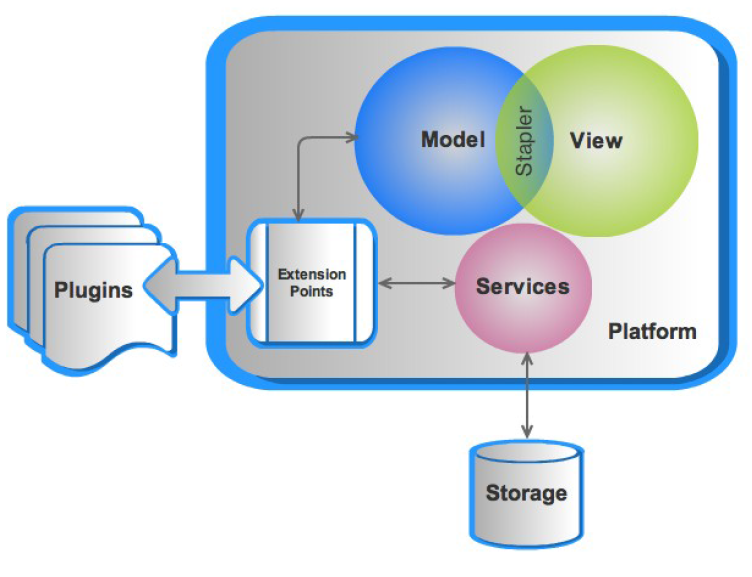
\includegraphics{img/jenkinsArchitecture.png}}
                    \caption{Přehled architektury serveru Jenkins CI \cite{architectureOverview}}
                    \label{imgJenkinsArchitecture}
                \end{center}
            \end{figure}     

    %%%%%%%%%%%%%%%%%%%%%%%%%%%%%%%%%%%%%%%%%%%%%%%%%%%%%%%%%%%%%%%%%%%%%%%%%%%%%%%%%%%%%%%%%%%%%%%
    \section{Webový server a servlet kontejner} \label{servletWebserver}
        V této kapitole jsou vysvětleny pojmy webový server a servlet kontejner, které se 
        na mnoha místech této práce objevují. Porozumění těmto pojmům je důležité, protože bez
        jejich znalosti by následující kapitoly byly obtížněji pochopitelné pochopitelné.
        
        Informace zde uvedené byly čerpány z článku \cite{webserverVsServletPage}.

        \subsection{Webový server}
            Webový server je program, který zprostředkovává komunikaci přes síť s klienty, kteří
            se k němu připojí a požadují po něm nějaká data. Tato komunikace probíhá pomocí protokolu \emph{HTTP}, 
            který je založen na modelu \emph{požadavek-odpověd} (anglicky \emph{request-response}).
            Model této komunikace je zachycen na obrázku \ref{imgWebserver}.
            
            Typický způsob komunikace webového serveru je, 
            že klient pomocí URL adresy specifikuje požadavek na nějaká
            data a server v odpovědi tato data pošle. Pokud by neexistoval za webovým serverem nějaký další
            program, tak by webový server vždy odpovídal na stejný požadavek stále stejnou odpovědí.

            \begin{figure}[ht]
                \begin{center}
                    \scalebox{0.63}{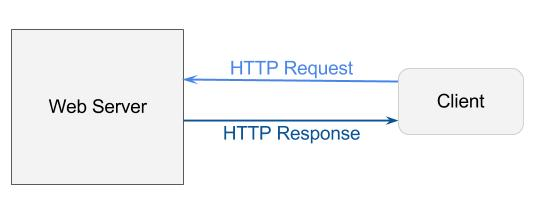
\includegraphics{img/web-server.jpg}}
                    \caption{Model komunikace webového serveru s klientem \cite{webserverVsServletPage}}
                    \label{imgWebserver}
                \end{center}
            \end{figure}

        \subsection{Servlet kontejner}
            Jelikož dostávat stále stejná statická data při stejném požadavku není dostatečná funkcionalita serveru,
            tak existují způsoby jak zajistit dynamickou práci s daty na serveru (a tudíž i měnící se odpovědi na stejný dotaz).
            Jedním ze způsobů jak této činnosti docílit je využití tzv. \emph{servletů},
            které jsou navrženy pro programovací jazyk Java.

            Servlet je standardní program (konkrétně jedna třída) napsaný v jazyce Java, 
            který implementuje rozhraní \texttt{javax.servlet}.
            Implementace tohoto rozhraní ho zavazuje k definování několika metod, ale jinak se jedná o běžnou
            třídu z které jsou při zpracovávání požadavků vytvářeny její instance.

            Základní myšlenkou servlet kontejneru je umožnit dynamicky vytvářet odpovědi (často webové stránky)
            pomocí vykonávání servletů. Samotný servlet kontejner je program, který poskytuje běhové prostředí pro vykonávání servletů,
            zajišťuje jejich vytváření, vykonávání a odstraňování. Dále se také podílí na zpracovávání HTTP požadavků, které jsou
            mu předávány od webového serveru. 

            Popsaný způsob fungování servlet kontejneru je znázorněn na obrázku \ref{imgServlet}.
            %teoreticky bych mohl dopsat něco o způsobu vyhodnocení servletu, ale to asi není podstatné
            \begin{figure}[ht]
                \begin{center}
                    \scalebox{0.75}{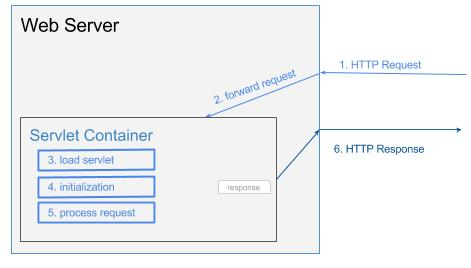
\includegraphics{img/servlet-container-life-cycle.jpg}}
                    \caption{Ukázka způsobu činnosti servlet kontejneru a jeho spolupráce s webovým serverem \cite{webserverVsServletPage}}
                    \label{imgServlet}
                \end{center}
            \end{figure}


         
    %%%%%%%%%%%%%%%%%%%%%%%%%%%%%%%%%%%%%%%%%%%%%%%%%%%%%%%%%%%%%%%%%%%%%%%%%%%%%%%%%%%%%%%%%%%%%%%
    \section{Nástroj Maven} \label{maven}
        Základní obecné informace, něco o pomkách - co tam najdeme, způsobech překladů
        \cite{mavenWeb}

    %%%%%%%%%%%%%%%%%%%%%%%%%%%%%%%%%%%%%%%%%%%%%%%%%%%%%%%%%%%%%%%%%%%%%%%%%%%%%%%%%%%%%%%%%%%%%%%
    \section{Server Jetty} \label{jetty}
        Jednou z komponent, které jsou aktuálně integrovány do serveru Jenkins CI, je webový server Jetty.
        Tento server je open source projektem vyvíjeným pod licencemi 
        Eclipse\footnote{Licence Eclipse je dostupná na adrese \texttt{http://www.eclipse.org/legal/epl-v10.html}} a
        Apache\footnote{Licence Apache je dostupná 
        na adrese \texttt{http://www.apache.org/licenses/LICENSE-2.0.html}}. 
        Je využíván velkým množstvím nástrojů jako jsou například \emph{Eclipse IDE}\footnote{Webové stránky nástroje Eclipse IDE 
        \texttt{http://www.eclipse.org/}} nebo \emph{Google AppEngine}\footnote{Webové stránky platformy Google AppEngine
        \texttt{https://developers.google.com/appengine/}}.

        Jetty je webový server a poskytuje funkcionalitu servlet kontejneru dle specifikace verze 3.0. 
        Je jej možné využít také jako webového klienta pro komunikaci se servery. Komunikace
        klientů i serverů využívajících Jetty probíhá asynchronně. 
        Návrh serveru umožňuje samostatné spouštění aplikací i jeho integraci do jiné aplikace. 

        Kromě těchto základních možností obsahuje
        řadu souvisejících technologií jako jsou SPDY, webové sokety\footnote{Oficiální stránky 
            specifikace webových soketů: \texttt{http://www.websocket.org/}}(angl. \emph{websocket}),
        JNDI, OSGi, JMX a další. 
        Informace v této kapitole byly čerpány z webových stránek serveru Jetty \cite{jettyWeb}, kde lze nalézt 
        další informace o zmíněných technologiích a o tomto serveru.
        
        Aktuální využití serveru Jetty v aplikaci Jenkins CI je podrobněji rozebráno
        v kapitole \ref{vyvojWinstone} a jeho srovnáním se serverem Undertow se 
        zabývá kapitola \ref{srovnani}.
        

    %%%%%%%%%%%%%%%%%%%%%%%%%%%%%%%%%%%%%%%%%%%%%%%%%%%%%%%%%%%%%%%%%%%%%%%%%%%%%%%%%%%%%%%%%%%%%%%
    \section{Servlet kontejner Winstone} \label{winstone}
        Další komponentou serveru Jenkins CI je servlet kontejner Winstone.
        Winstone je velmi jednoduchý a poskytuje funkcionalitu
        servlet kontejneru aniž by byl zatížen velkým množstvím požadavků, které jsou ve specifikaci jazyka Java EE.
        Nikdy neposkytoval veškeré služby servlet kontejneru, které specifikace jazykPlugins are responsible for a definuje. 
        V jeho názvu je zahrnutý pouze pojem servlet kontejner, ale tato aplikace vykonává i služby
        webového serveru odpovídající popisu v kapitole \ref{servletWebserver}.

        Hlavními cíli projektu bylo poskytovat funkcionalitu servlet kontejneru pouze pro jednu aplikaci,
        což je opačný přístup než u běžných aplikačních serverů jako jsou Glasfish, JBoss, aj.
        Díky jeho omezeným službám je jeho velikost velmi malá a umožňuje jednoduchou integraci s
        cílovou aplikací.

        Uvedené informace byly čerpány z oficiální stránky projektu Winstone \cite{winstoneWeb}.

        \subsection{Nedostatky servlet kontejneru Winstone}
            Původní myšlenka jednoduchého servlet kontejneru byla pro projekt Jenkins CI zajímavá.
            Kontejner Winstone má několik zásadních nedostatků kvůli kterým bylo časem jeho využití v 
            Jenkins CI problematické \cite{kohsukeTopic}. 

            Vývoj projektu Winstone již před delší dobou ustal a tím pádem nebyla poskytována 
            žádná další podpora pro řešení a opravování objevených nedostatků a chyb. 
            Značné množství bezpečnostních chyb objevených v projektu Jenkins CI bylo právě
            způsobeno tímto servlet kontejnerem.

            Zpočátku možnosti servlet kontejneru postačovaly, ale časem je potřeba, aby 
            byly přidávány nové funkcionality, které odpovídají aktuálním trendům a 
            novým specifikacím. Příkladem mohou být nové specifikace servlet kontejneru,
            vývoj nových technologií jako webové sokety.


    %%%%%%%%%%%%%%%%%%%%%%%%%%%%%%%%%%%%%%%%%%%%%%%%%%%%%%%%%%%%%%%%%%%%%%%%%%%%%%%%%%%%%%%%%%%%%%%
    \section{Vývoj servlet kontejneru v komunitě Jenkins CI} \label{vyvojWinstone}
        Po ukončení vývoje projektu Winstone se musela o jeho potřebné úpravy starat komunita
        Jenkins CI. Takováto práce je pro komunitu velmi zatěžující
        a naprosto neefektivní. Byly prováděny především nutné opravy bezpečnostních chyb v kontejneru,
        ale jinak aplikace dále degenerovala. Pro tento vývoj vznikl v projektu Jenkins CI nový 
        repozitář, který vycházel z původní verze servlet kontejneru 
        Winstone\footnote{Repozitář, kde komunita Jenkins CI provádí úpravy projektu Winstone:
        \texttt{https://github.com/jenkinsci/winstone}}. Z tohoto zdroje
        a z článku o integraci Jetty s kontejnerem Winstone \cite{kohsukeTopic} jsou čerpány uváděné informace. 
        
        \medskip
        Vývoj původního servlet kontejneru Winstone probíhal uvedeným způsobem 
        až do verze \emph{0.9.10-jenkins-47}. Následně byl tento způsob vývoje zastaven
        a do kontejneru Winstone byl integrován webový server a servlet kontejner
        Jetty. Tímto krokem vznikla 
        interní verze servlet kontejneru \emph{Winstone 2.0}. Velká část kódu 
        kontejneru Winstone byla odstraněna a veškerá činnost webového serveru a servlet 
        kontejneru je nyní vykonávána pomocí serveru Jetty. Z původního kontejneru Winstone
        zůstal způsob zpracovávání a nastavování parametrů. 
        Tato změna proběhla poměrně narychlo
        a nebyla detailně otestována. Obsahuje zřejmě ještě množství nepotřebného kódu a 
        samotná implementace není moc předhledná.

        
        %%%%%%%%%%%%%% DŮLEŽITÉ KONTROLOVAT SMYSL %%%%%%%%%%%%%%%%%%%%
        \medskip
        Těsně před integrací serveru Jetty s Jenkins CI
        vznikalo zadání tohoto diplomového projektu, které mělo za cíl
        výrazně zlepšit aktuální stav servlet kontejneru v projektu Jenkins CI. Během
        formulace zadání byl servlet kontejner v projektu přepracován a proto
        muselo být zadání upraveno. I po této změně byly stále důvody pro 
        nahrazení stávajícího servlet kontejneru serverem Undertow.
        Aktuální situace již není tak kritická jako v předchozí verzi,
        ale může přinést ještě další zlepšení.
                

    %%%%%%%%%%%%%%%%%%%%%%%%%%%%%%%%%%%%%%%%%%%%%%%%%%%%%%%%%%%%%%%%%%%%%%%%%%%%%%%%%%%%%%%%%%%%%%%
    \section{Server Undertow} \label{undertow}
        Obecné informace, k čemu je dobrý, srovnání s Jetty, odkazy na výsledky testování výkonu

        Jak se používá, jak se s ním pracuje a programuje, detailněji
         argumenty v pdfku k wildfly8 - bezpecnost, rychlost, ...
        \cite{undertowWeb}

        \subsection{Srovnání serverů Undertow a Jetty}\label{srovnani}
            Stávající servlet kontejner v Jenkins CI je sice tvořen
            kombinací kontejneru Winstone a serveru Jetty, ale veškerou
            časově kriticky náročnou práci při běhu aplikace vykonává server
            Jetty. Proto pokud chceme srovnávat aktuální řešení servlet kontejneru
            v Jenkins CI, tak bychom měli srovnávat server Jetty se serverem Undertow.

            \medskip
            Budeme tedy srovnávat servery Undertow a Jetty a jejich výhody a nevýhody
            vzhledem k využití v systému Jenkins CI:
            \begin{itemize}
                \item {\textbf{Rychlost:} Server Undertow je aktuálně ještě stále ve verzi \emph{beta}, ale už přesto existují
                    testy, které prokazují, že je výkonnější než server Jetty. V tomto           
                    testování\footnote{Porovnání rychlosti, odezvy a celkové výkonnosti serverů Undertow, Jetty a jiných: 
                    \\\texttt{http://www.techempower.com/benchmarks/\#section=data-r8\&hw=ec2\&test=plaintext}}
                    byl server Undertow i více 3,5 krát rychlejší než server Jetty a dosahoval menší
                    až třetinové odezvy.
            
            Na obrá
        
                    Po dokončení diplomového projektu a provedení plánované
                    integrace uskutečním vlastní porovnání těchto dvou implementací a pokusím se potvrdit
                    tyto výsledky.}

                \item{\textbf{Spolehlivost:} Dalším důležitým aspektem je spolehlivost daného serveru. 
                        Server Jetty má za sebou již dlouhou historii a je integrován ve velkém množství
                        různých aplikací\footnote{Aplikace, které využívají server Jetty: \texttt{http://www.eclipse.org/jetty/powered/}},
                        což mu dodává velkou důvěryhodnost a lze očekávat, že bude pracovat velmi 
                        spolehlivě. 
                        
                        U server Undertow ještě nebyla dokončena první finální verze,
                        takže lze předpokládat, že může obsahovat ještě drobné nedostatky,
                        které budou časem opravovány. Jelikož tento server bude integrován
                        v novém aplikačním serveru WildFly 8, tak lze předpokládat,
                        že postupem času bude také velmi spolehlivý. 
                        Nicméně v tomto aspektu je server Jetty zřejmě 
                        aktuálně lepší.}

                \item{\textbf{Rychlost spuštění:}  Velmi často je u serverů hodnocena hlavně
                    jejich rychlost a výkonnost v zátěži. Je běžné, že nebývá kladen důraz na
                    velmi rychlé spuštění serveru. Pro standardní běh serveru, kdy bývá 
                    spuštěn jednou za několik týdnů či měsíců po nějakých úpravám aplikace,
                    není doba spuštění zásadní. Pokud se na to podíváme z pohledu testování
                    aplikace, kdy jsou spouštěny integrační testy a pro každý test musí být
                    znovu spuštěn server, tak je rychlost nastartování serveru velmi podstatná.
                    
                    Cílem serveru Undertow je být minimalistickým a velmi rychlým 
                    řešením. Server Jetty poskytuje kvalitní podporu pro běh aplikací, ale je 
                    rozsáhlejší a není jeho prioritou, aby byl extrémně rychle spuštěn.
                    Lze usuzovat, že rychlost spuštění bude u serveru Undertow výrazně nižší
                    než u serveru Jetty. Tato skutečnost bude testována při vyhodnocování
                    výsledků této diplomové práce.

                    V aktuálním stavu Jenkins CI běží integrační testy více než hodinu. Pokud 
                    by byl servlet kontejner spuštěn za poloviční dobu, tak by mohla být doba testování
                    zkrácená také téměř na polovinu.

                    }

                \item{\textbf{Velikost:} Jelikož je servlet kontejner přímo integrován do archivu ve kterém
                    je systém Jenkins CI distribuován, tak komunita dbá na to, aby přidávané komponenty
                    nebyly příliš velké. Z důvodu velikosti byla v minulosti zavržena například
                    myšlenka využít aplikační server \emph{JBoss AS 7} jako náhradu za kontejner
                    Winstone\footnote{Diskuze o velikosti archivu Jenkins CI: \texttt{link}}. %TODO link
                    
                    Po integraci Jetty vzrostla velikost servlet kontejneru o 1,5 MB na celkovou
                    velikost 1,8 MB. U serveru Undertow je uváděno, že jeho archiv má méně
                    než 1 MB a konečná velikost po integraci bude také záležet na využitých komponentách
                    a rozsahu implementace. Přesto z pohledu velikosti výsledného archivu
                    se jeví server Undertow jako výhodnější, ale rozdíl oproti serveru Jetty není zásadní.
                    Rozdíl je zřejmě přibližně 1MB, což jsou necelé 2\% z aktuální velikosti
                    Jenkins CI\footnote{Stránka, kde je v systému Jenkins CI automatizovaně
                    sledována velikost archivu aplikace:\\ 
                    \texttt{https://wiki.jenkins-ci.org/display/JENKINS/Jenkins+WAR+Size+Tracker}}.}

                %Tato část by měla být pečlivě překontrolována
                \item{\textbf{Konfigurovatelnost:} Server Undertow je velmi flexibilní a způsob
                    jeho návrhu, který byl popsán výše, umožňuje provádět mnoho různých úpravy 
                    své činnosti dle potřeby a využít pouze ty části, které potřebujeme.
                    Tato filozofie je velmi blízká filozofii projektu Jenkins CI. 
                    
                    Server Jetty
                    je oproti tomu robustnější a rozsáhlejší, ale neumožňuje tak velké přizpůsobování potřebám
                    uživatele jako například využití jen několika malých částí jeho funkčnosti či jejich
                    kombinování. }

            \end{itemize}
        

%%%%%%%%%%%%%%%%%%%%%%%%%%%%%%%%%%%%%%%%%%%%%%%%%%%%%%%%%%%%%%%%%%%%%%%%%%%%%%%%%%%%%%%%%%%%%%%

%%%%%%%%%%%%%%%%%%%%%%%%%%%%%%%%%%%%%%%%%%%%%%%%%%%%%%%%%%%%%%%%%%%%%%%%%%%%%%%%%%%%%%%%%%%%%%%
\chapter{Analýza současného stavu a návrh integrace}
    většina informací čerpána přímo ze zdrojových kódu aplikace a komponent Jenkins CI.
    
    \section{Aktuální stav architektury servlet kontejneru v~Jenkins~CI}
        V následujících dvou podkapitolách bude blíže analyzována architektura
        Jenkins CI z pohledu servlet kontejneru. Tato analýza je velmi důležitá
        pro pochopení návazností jednotlivých komponent, které budou později upravovány.

        Jak již bylo uvedeno v kapitole \ref{vyvojWinstone}, současný servlet kontejner 
        v Jenkins CI se skládá z nástojů Winstone a Jetty, které byly popisovány v 
        předchozí kapitole. Velká část servlet
        kontejneru Winstone byla odstraněna a zůstala pouze část, která
        provádí zpracování parametrů
        programu po spuštění aplikace. Činnost webového serveru, servlet kontejneru
        a další vykonává server Jetty.
        

        \subsection{Architektura Jenkins CI z pohledu servlet kontejneru}
            Na vysoké úrovni pohledu lze architekturu serveru Jenkins CI rozdělit do tří částí:
            
            \begin{itemize}
                \item{\textbf{Jádro aplikace} do kterého patřím nejnutnější základní komponenty systému,
                    části, které jsou pro Jenkins CI specifické a vznikaly a vznikají v rámci tohoto projektu.}

                \item{\textbf{Přídavné moduly} aplikace, které jsou do ní dynamicky přidávány jako archivy javových programů
                    \texttt{.jar}. Tyto součásti jsou většinou nutné pro standardní běh aplikace a je s nimi aplikace
                    běžně dodávána (teoreticky lze
                    aplikaci spustit např. bez servlet kontejneru pomocí aplikačního serveru, ale toto je spíše ojedinělý případ). 
                    
                    Komponenty z této kategorie pocházejí typicky z externích projektů.
                    Do této kategorie také spadá servlet kontejner, který je aktuálně do aplikace
                    přidáván pod názvem \texttt{winstone.jar}.}

                \item{\textbf{Rozšiřující moduly} (angl. plugins) jsou samostatné menší programy, které nějakým
                    způsobem přidávají funkcionalitu serveru Jenkins CI. Typicky nejsou dodávány s aplikací
                    a uživatel si je může stáhnout popř. si nějaký vlastní modul vytvořit.
                    
                    Samotná aplikace se dodává jen s těmi nejnutnějšími součástmi a ponechává na uživatelích, které
                    další funkcionality si do systému doinstalují. V současné době již existují stovky takových
                    modulů, které jsou volně ke stažení. }
            \end{itemize}
            

            V následujícím textu bude při popisu interních součástí zdrojových kódů použita notace
            ve tvaru \texttt{Název\_třídy::Název\_metody}.

            Architektura Jenkins CI z pohledu servlet kontejneru je znázorněna na obrázku \ref{imgArchitekturaServlet}.
            Jsou zde zachyceny především komponenty, které přímo souvisejí s činností servlet kontejneru.

            \begin{figure}[h!t]
                \begin{center}
                    \scalebox{0.63}{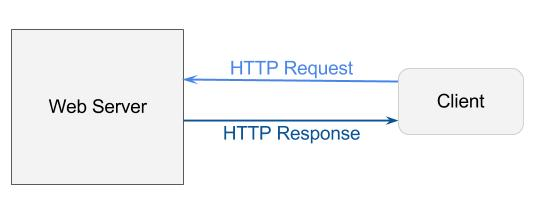
\includegraphics{img/web-server.jpg}}
                    \caption{Přehled architektury systému Jenkins CI z pohledu vestavěného servlet kontejneru}
                    \label{imgArchitekturaServlet}
                \end{center}
            \end{figure}

            
            Archiv \texttt{winstone.jar} obsahuje servlet kontejner pro Jenkins CI. Název je nyní sice mírně matoucí
            (způsoben předchozí implementací, ale aktuálně jsou součástí tohoto archivu komponenty Winstone a Jetty.

            Velmi podstatnu součásti aplikace z pohledu servlet kontejneru je komponenta\\\texttt{extras-executable-war}. 
            Tato součást aplikace je sice malá, ale obsahuje metodu \texttt{main}, kterou se aplikace spouští 
            (pokud není spuštěna v aplikačním serveru). Hlavním úkolem této komponenty je právě spustit 
            servlet kontejner a tím spustit i celou aplikaci. Tento proces spuštění aplikace je zobrazen
            na obrázku \ref{imgArchitekturaSpusteni}.

            Nejprve je spuštěna vstupní metoda celé aplikace \texttt{Main.java::main} z komponenty\\\texttt{extras-executable-war}.
            Po počáteční inicializaci je předáno řízení aplikace metodě \\\texttt{Launcher.java::main}
            z archivu \texttt{winstone.jar}, která provede nastartování a 
            zavedení servlet kontejneru. Následně je provedena inicializace a spuštění
            jediného servletu aplikace Jenkins CI a tím je servlet Stapler. %TODO reference na stapler
            Pokud se podaří úspěšně spustit tento servlet, tak je spuštění celé aplikace Jenkins CI z pohledu
            servlet kontejneru úspěšně hotovo a aplikace běží.

            \begin{figure}[h!t]
                \begin{center}
                    \scalebox{0.63}{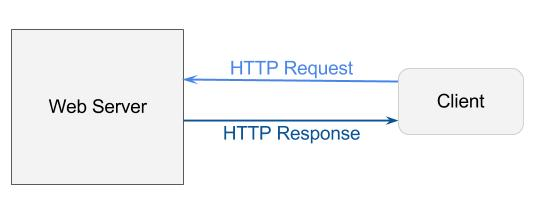
\includegraphics{img/web-server.jpg}}
                    \caption{Průběh spouštění aplikace Jekins CI při spouštění pomocí vestavěného servlet kontejneru}
                    \label{imgArchitekturaSpusteni}
                \end{center}
            \end{figure}


        \subsection{Průběh komunikace prostřednictvím servlet kontejneru}
            Po úspěšném zavedení a spuštění aplikace provádí servlet kontejner
            zpracovávání příchozích požadavků a předává je aplikaci Jenkins CI. 
            Typický zobecněný průběh komunikace servlet kontejneru s aplikací je znázorněn
            na obrázku \ref{imgKomunikace}. 

            \begin{figure}[h!t]
                \begin{center}
                    \scalebox{0.63}{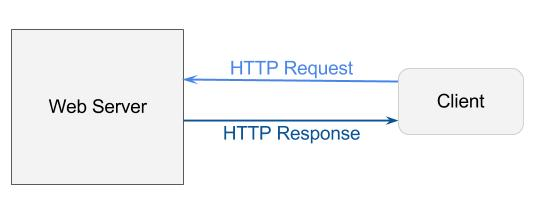
\includegraphics{img/web-server.jpg}}
                    \caption{Průběh komunikace aplikace Jekins CI prostřednictvím vestavěného servlet kontejneru}
                    \label{imgArchitekturaSpusteni}
                \end{center}
            \end{figure}

            Při komunikaci je příchozí HTTP požadavek zpracován pomocí servlet kontejneru 
            a následně předán patřičnému servletu (dle nastavení pravidel pro směřování požadavků).
            Jelikož je v aplikaci pouze jediný servlet Stapler, tak je požadavek předán jemu.
            Tato komponenta následně provede netriviálním způsobem rozhodnutí, které
            části aplikace předat požadavek k vykonání  nebo zda náleží nějakému rozšiřujícímu modulu.
            Následně obráceným postupem probíhá zaslání HTTP odpovědi klientovi.

            Je zde zachycena pouze jedna z možných činností
            servlet kontejneru a tou je zpracovávání komunikace protokolem HTTTP. 
            Další činnosti kontejneru budou rozebírány později.

 


    \section{Zpětná kompatibilita}
        zachování funkčnosti parametrů - závisí na tom různé komponenty a pluginy Jenkins. 
        Odcitovat Keysukeho článek na docs.gmail.  
        
        Možnost řízení security věcí -- \cite{securityArchitecture}, \cite{securityArchitectureWinstone}
        komunikace přes HTTP
        komunikace přes HTTPS
        AJP13     
        SPDY - aktuálně není v Jenkins využíván, pouze je podporován Jetty

        %parametry aspon do přílohy

        \subsection{Zjištěné problémy}
            Rozdílná verze Javy - Undertow v. 7, Jenkins v. 6 => nutnost převést Jenkins na verzi 7,
            což mírně omezuje okamžité využití v hlavní větvi, ale do budoucna určitě bude nějaký přechod


    \section{Zvolení způsobu integrace serveru Undertow}
        Způsob vyhodnocení správnosti výsledného řešení pomocí testů jenkins

        \subsection{Varianta ponechání Winstonu}

        \subsection{Varianta nahrazení Jetty i Winstonu}





\chapter{Závěr}
    Zhodnocení aktuálního stavu a budoucí výhled a plán

%=========================================================================




